% HF-Digital Twin Platform - IEEE Format Research Paper
\documentclass[conference]{IEEEtran}
\IEEEoverridecommandlockouts
\usepackage{amsmath,amssymb,amsfonts}
\usepackage{cite}
\usepackage{url}
\usepackage{booktabs}
\usepackage{multirow}
\usepackage{array}
\usepackage{graphicx}
\usepackage{float}
\usepackage{subcaption}
\usepackage{tikz}
\usetikzlibrary{shapes.geometric, arrows.meta, positioning, calc}
\usepackage{textcomp}
\usepackage{xcolor}
\usepackage[utf8]{inputenc}

\def\BibTeX{{\rm B\kern-.05em{\sc i\kern-.025em b}\kern-.08em T\kern-.1667em\lower.7ex\hbox{E}\kern-.125emX}}

\begin{document}

\title{HF-Digital Twin Platform: A Hybrid Mechanistic--ML System for Personalized Heart Failure Medication Recommendations and Clinical Data Integration}

\author{
\IEEEauthorblockA{
\begin{tabular}{cc}
\textbf{Pratik Kumar\textsuperscript{1}} & \textbf{Thakur Chand Choudhary\textsuperscript{2}} \\
Department of Sensor and Biomedical Engineering & Department of Sensor and Biomedical Engineering \\
Vellore Institute of Technology (VIT) & Vellore Institute of Technology (VIT) \\
Vellore, Tamil Nadu, India & Vellore, Tamil Nadu, India \\
\texttt{pratik.kumar2024a@vitstudent.ac.in} & \texttt{thakur.chand2024@vitstudent.ac.in} \\
\\
\multicolumn{2}{c}{\textbf{Dr. Muthu Raja S\textsuperscript{*}}} \\
\multicolumn{2}{c}{School of Electronic Engineering} \\
\multicolumn{2}{c}{Vellore Institute of Technology (VIT)} \\
\multicolumn{2}{c}{Vellore, Tamil Nadu, India} \\
\multicolumn{2}{c}{\texttt{muthurajas@vit.ac.in}} \\
\end{tabular}
}
}

\maketitle

\begin{abstract}
Heart failure (HF) management requires personalized medication selection from a large space of drugs and combinations, aligned with guidelines and patient-specific physiology. We present the HF-Digital Twin Platform, a hospital-grade system that combines data-driven machine learning with mechanistic cardiovascular models to deliver drug-level recommendations, combination success prediction, and longitudinal patient modeling. The platform integrates a calibrated digital twin (per-patient Windkessel calibration and outcome-based updates), an RxNorm-backed medication database, a clinical document pipeline (OCR, prescription and lab parsing, temporal extraction into a structured patient database), and a production REST API with a professional web frontend. We describe the architecture, implementation, validation strategy, and design choices that avoid mock or placeholder outputs when models are untrained or data are incomplete. The system is evaluated on its modular design, alignment with clinical workflows, and technical complexity spanning ML, mechanistic modeling, and clinical data engineering. The paper provides full technical detail on data schema, API design, model formulation, and safety measures to support reproducibility and deployment in research or pilot clinical settings.
\end{abstract}

\begin{IEEEkeywords}
Digital twin, heart failure, personalized medicine, medication recommendation, mechanistic model, machine learning, RxNorm, clinical decision support, Windkessel model, treatment comparison.
\end{IEEEkeywords}

\section{Introduction}
\IEEEPARstart{H}{eart} failure (HF) is a leading cause of morbidity and mortality, with guideline-directed medical therapy (GDMT) involving multiple drug classes, titrations, and combination strategies~\cite{heidenreich2022aha,mcdonagh2021esc}. Individual response varies widely, and the space of possible regimens is large. Clinical decision support that can recommend specific drugs and dosages, predict combination success, and adapt to observed outcomes would support personalized care while remaining interpretable and auditable. Building such a system requires integrating population-level evidence (from trials and registries), patient-level data (demographics, vitals, labs, medications, and outcomes), and physiological models that can be calibrated to the individual. It also requires strict safeguards so that the system never presents fabricated or default recommendations when the underlying models are not trained or when inputs are incomplete.

Digital twins in healthcare aim to maintain a dynamic, calibrated representation of an individual patient for prediction and optimization~\cite{grieves2014digital,barricelli2019digital}. Most prior work either relies on population-level ML alone or on mechanistic models without patient-specific calibration and learning. A hybrid approach---combining data-driven models trained on cohorts with physics-based cardiovascular models calibrated to the individual---can improve both personalization and interpretability~\cite{topol2019high,rajkomar2019scalable}.

We present the \textbf{HF-Digital Twin Platform}: a full-stack system that (1) provides \emph{drug-level} recommendations (specific medications, dosages, strengths, frequencies) and combination success rates; (2) maintains a \emph{patient digital twin} via Windkessel calibration and outcome-based model updates; (3) ingests clinical documents (PDFs/images) through OCR and structured parsing into a temporal patient database; and (4) exposes a production API and hospital-grade web UI with strict validation so that untrained models or incomplete data never produce fictitious recommendations~\cite{ghassemi2021practical}.

The main contributions are: (a) an integrated architecture that combines ML recommenders, a combination success predictor, a mechanistic calibrator, and RxNorm-based medication knowledge; (b) a clinical data pipeline from raw documents to time-series labs and vitals; (c) design and implementation details suitable for reproducibility; and (d) evaluation of the system's complexity and alignment with clinical use.

\subsection{Problem Scope and Objectives}
The target user is a clinician or researcher managing heart failure patients: the system must support entry of demographics, vitals, labs, and comorbidities; ingestion of historical documents (prescriptions, lab reports) to build a longitudinal record; and retrieval of actionable recommendations (specific drugs, dosages, and combination success estimates) without ever returning fabricated or placeholder results when the model is not trained or inputs are incomplete. A secondary objective is to maintain a patient-specific digital twin that can be calibrated from observed data and updated when real outcomes become available, bridging population-level evidence with individual physiology.

\section{Related Work}

This section reviews prior and concurrent work on digital twins in healthcare, heart failure guidelines and medication knowledge bases, machine learning for medication and outcomes, mechanistic cardiovascular models, document understanding for clinical data, safety and validation in clinical ML, and clinical decision support. We then position our contribution relative to identified gaps.

\subsection{Digital Twins in Healthcare}
Digital twins were first formalized in manufacturing and complex systems to maintain a synchronized digital representation of a physical asset for prediction and optimization~\cite{grieves2014digital}. Barricelli et al.~\cite{barricelli2019digital} provide a survey of definitions, characteristics, and design implications across domains; they characterize digital twins by lifecycle (design, deployment, operation) and by the degree of data coupling between the physical and digital entities. Lee et al.~\cite{lee2020digital} discuss cyber-physical architectures that link physical processes to digital models, a pattern that transfers to patient-level modeling. In healthcare specifically, Lauretani et al.~\cite{lauretani2020digital} review applications of digital twins and highlight lessons learned and open issues, including the need for interpretability and integration with clinical workflows. Our platform implements an \emph{operational} twin: initialized from patient data, calibrated with mechanistic models (Windkessel), and updated from observed outcomes, thus combining the lifecycle view of~\cite{barricelli2019digital} with a healthcare-specific focus on medication and physiology~\cite{lauretani2020digital}.

\subsection{Heart Failure Guidelines and Medication Space}
Contemporary heart failure guidelines define evidence-based drug classes and combination strategies. The 2022 AHA/ACC/HFSA guideline~\cite{heidenreich2022aha} and the 2021 ESC guideline~\cite{mcdonagh2021esc} recommend ACE inhibitors, ARBs, ARNI, beta-blockers, MRAs, SGLT2 inhibitors, and others, with explicit guidance on titration and combination therapy. ESC position papers also address comorbidities and frailty~\cite{ambrosetti2021esc}, which affect medication choices. To support \emph{specific} drug and dosage recommendations (rather than category-level only), standardized terminologies are required. RxNorm~\cite{nelson2002rxnorm} provides normalized names and concept identifiers for clinical drugs and is widely used in EHR and medication reconciliation~\cite{sterling2016rxnorm}; the RxNorm API~\cite{rxnormapi} enables programmatic lookup of properties, strengths, and interactions. Our platform aligns with guideline categories while resolving to specific drugs and dosages via RxNorm and an internal medication database, supporting both guideline adherence and granular, actionable output.

\subsection{Machine Learning for Medication and Outcomes}
Machine learning for medication recommendation and outcome prediction has been applied to electronic health records and trial data~\cite{rajkomar2019scalable}. Topol~\cite{topol2019high} discusses the convergence of human and artificial intelligence in high-performance medicine and stresses the need for interpretability and validation. In cardiovascular medicine, Shameer et al.~\cite{shameer2018mlhf} review ML applications and note that heart failure prediction and treatment optimization are active areas. Chicco and Jurman~\cite{chicco2020uci} demonstrated that ML can predict survival of heart failure patients from limited features (e.g., serum creatinine and ejection fraction) using the UCI Heart Failure dataset. Komorowski et al.~\cite{komorowski2018ai} learned treatment strategies for sepsis in intensive care from MIMIC data, illustrating reinforcement-learning-style optimization over treatment sequences. MIMIC-III~\cite{johnson2016mimic} remains a key resource for temporal and critical-care modeling. Our system uses Random Forest and Gradient Boosting~\cite{breiman2001random,friedman2001greedy} for medication selection and treatment effect prediction, implemented with scikit-learn~\cite{scikit}, and adds a dedicated \emph{combination} success predictor and drug-level resolution rather than category-level only.

\subsection{Mechanistic Cardiovascular Models}
Mechanistic models provide interpretable, physics-based representations of physiology. The Windkessel model approximates arterial pressure from cardiac output using resistance $R$ and compliance $C$; Westerhof et al.~\cite{westerhof2009arterial} give a clear treatment of the arterial windkessel and its role in hemodynamics. Such models are well-suited to per-patient calibration because the parameters have direct physiological meaning. Many ML-for-healthcare systems are purely data-driven and lack this interpretable layer~\cite{rajkomar2019scalable}; combining mechanistic models with ML can improve both personalization and explainability~\cite{topol2019high}. We use a two-element Windkessel with ODE $dP/dt = (CO(t) - P/R)/C$, calibrating $R$ and $C$ to patient history via numerical optimization and updating them from observed outcomes, so that the digital twin maintains a patient-specific physiological component alongside the data-driven recommender.

\subsection{Document Understanding and Clinical Data}
Structured extraction from prescriptions and lab reports supports medication reconciliation and longitudinal analytics. Sterling et al.~\cite{sterling2016rxnorm} use structured and unstructured data to identify patients' need for formal medication reconciliation, highlighting the role of document-derived data in clinical workflows. OCR is a prerequisite: Tesseract~\cite{tesseract} is a widely used open-source engine, and EasyOCR~\cite{easyocr} provides a ready-to-use alternative with broad language support. Our pipeline uses both, with custom parsers for prescriptions and lab values and a temporal PDF parser that aggregates multi-page documents into time-series labs and vitals stored in the clinical database, aligning with the need to turn documents into actionable, queryable data~\cite{sterling2016rxnorm}.

\subsection{Safety and Validation in Clinical ML}
Deploying AI on healthcare data requires rigorous validation and clear failure modes. Ghassemi et al.~\cite{ghassemi2021practical} provide practical guidance on AI for healthcare data and emphasize that systems should fail safely and transparently when inputs are invalid or when models are not applicable. Bates et al.~\cite{bates2018cdss} discuss the potential of AI in healthcare and the importance of integrating with clinical workflows and maintaining auditability. Our platform enforces explicit validation: recommendations are returned only when the model is trained and required patient fields (e.g., age, ejection fraction) are present; otherwise the API returns HTTP 400 with a structured error message. This avoids the risk of presenting synthetic or default recommendations as if they were model-derived~\cite{ghassemi2021practical}.

\subsection{Clinical Decision Support and Workflow Integration}
Clinical decision support systems (CDSS) for medication must integrate with clinician workflows and provide actionable, interpretable output. Sutton et al.~\cite{sutton2020cdss} review CDSS benefits, risks, and strategies for success; Musen et al.~\cite{musen2014cdss} describe the design of clinical decision-support systems in the broader context of biomedical informatics. Wright et al.~\cite{wright2015medrec} discuss clinical decision support for medication management and note both opportunities and barriers to adoption. Explainability is a recurring theme: Miller~\cite{miller2018explanation} reviews explanation in AI from the perspective of the social sciences and argues that explanations should be tailored to the user and context. Our design keeps the UI minimal (dashboard plus a few main sections), reuses a single patient form across flows, and returns structured JSON with specific drugs, dosages, and combination success rates so that results are actionable and presentable in a consistent format~\cite{sutton2020cdss,wright2015medrec}. Documentation (API, user guide, technical docs) supports integration and training.

\subsection{Positioning and Gap}
Prior work has established digital twins in manufacturing and their survey in broader contexts~\cite{grieves2014digital,barricelli2019digital}, guidelines and RxNorm for HF medications~\cite{heidenreich2022aha,nelson2002rxnorm}, ML for HF and critical care~\cite{chicco2020uci,komorowski2018ai,johnson2016mimic}, Windkessel models for hemodynamics~\cite{westerhof2009arterial}, and safety and CDSS design principles~\cite{ghassemi2021practical,sutton2020cdss}. To our knowledge, no single system integrates (i) a calibrated patient digital twin with mechanistic (Windkessel) and ML components, (ii) drug-level and combination-level recommendations backed by RxNorm, (iii) a clinical document pipeline from PDFs to temporal labs/vitals, and (iv) strict validation that prevents any mock or placeholder recommendations when the model is untrained or inputs are incomplete. The HF-Digital Twin Platform fills this gap by providing an end-to-end, hospital-grade stack with the literature-backed design choices reviewed above.

\section{System Architecture and Methodology}

\subsection{High-Level Architecture}
Figure~\ref{fig:arch} shows the three-tier architecture: (1) \textbf{Frontend}---React/TypeScript with dashboard-driven navigation and reusable patient forms; (2) \textbf{API layer}---FastAPI~\cite{fastapi} with Pydantic~\cite{pydantic} validation and multiple routers (recommendations, documents, digital twin, temporal data, medications); (3) \textbf{Engine and data}---recommendation engine (medication recommender, effect predictor, combination success predictor, patient calibrator) and data layer (clinical patient database, medication database backed by RxNorm, model registry). Communication is synchronous over HTTP/JSON; the frontend does not assume WebSockets or server-sent events. The backend is stateless with respect to session; all patient state is stored in the databases so that scaling can be achieved by adding API workers behind a load balancer.

\subsection{Notation and Conventions}
In the Windkessel model, $P$ denotes arterial pressure, $CO$ cardiac output, $R$ systemic vascular resistance, and $C$ arterial compliance; time is $t$. For the ML components, $\mathbf{x}$ denotes the patient feature vector, $y$ the outcome (e.g., benefit indicator or continuous effect), and $\hat{y}$ the model prediction. Combination success is a scalar in $[0,1]$ predicted by the combination success predictor from $(\mathbf{x}, \mathcal{M})$ where $\mathcal{M}$ is the set of medication identifiers. All model outputs used for recommendations are produced only when the model is trained and inputs pass validation.

\begin{figure}[t]
\centering
\resizebox{\columnwidth}{!}{%
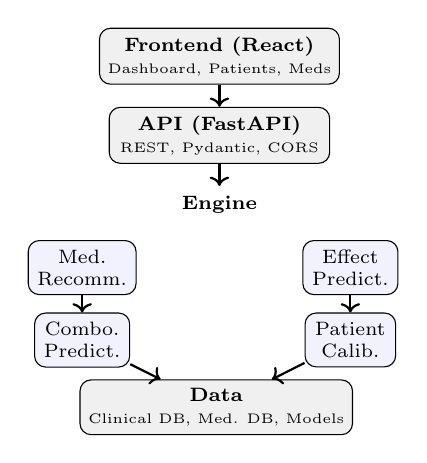
\begin{tikzpicture}[
  node distance=0.28cm and 0.5cm,
  box/.style={draw, rounded corners, fill=blue!5, minimum width=1.15cm, minimum height=0.45cm, font=\scriptsize, align=center},
  layer/.style={draw, rounded corners, fill=gray!12, inner sep=3pt, font=\scriptsize},
  arrow/.style={->, thick}]
  \node[layer, minimum width=2.8cm, align=center] (fe) {\textbf{Frontend (React)}\\{\tiny Dashboard, Patients, Meds}};
  \node[layer, below=of fe, minimum width=2.8cm, align=center] (api) {\textbf{API (FastAPI)}\\{\tiny REST, Pydantic, CORS}};
  \node[below=of api, align=center, font=\scriptsize] (eng) {\textbf{Engine}};
  \node[box, below left=0.22cm and 0.45cm of eng] (m) {Med.\\Recomm.};
  \node[box, below right=0.22cm and 0.45cm of eng] (e) {Effect\\Predict.};
  \node[box, below=0.22cm of m] (c) {Combo.\\Predict.};
  \node[box, below=0.22cm of e] (cal) {Patient\\Calib.};
  \node[layer, below=0.5cm of $(c)!0.5!(cal)$, minimum width=2.8cm, align=center] (data) {\textbf{Data}\\{\tiny Clinical DB, Med. DB, Models}};
  \draw[arrow] (fe) -- (api);
  \draw[arrow] (api) -- (eng);
  \draw[arrow] (m) -- (c);
  \draw[arrow] (e) -- (cal);
  \draw[arrow] (c) -- (data);
  \draw[arrow] (cal) -- (data);
\end{tikzpicture}%
}
\caption{High-level system architecture.}
\label{fig:arch}
\end{figure}

\subsection{Recommendation Pipeline}
The recommendation pipeline (Fig.~\ref{fig:flow}) enforces validation before any ML call: demographics and ejection fraction are required; the model must be trained. If validation fails, the API returns an explicit error instead of mock results. For valid requests, the flow is: ML recommendation $\rightarrow$ medication database lookup (specific drugs and dosages) $\rightarrow$ combination success predictor $\rightarrow$ output with drugs, dosages, and success rates. The ``standard'' recommendation path returns category-level suggestions and effect estimates; the ``enhanced'' path additionally resolves to specific RxNorm-backed drugs, strengths, dosage forms, and frequencies, and attaches a predicted combination success rate (0--1) and expected outcomes (e.g., ejection fraction change, mortality risk reduction). Both paths use the same validation gate so that neither can return results when the model is untrained or required fields are missing.

\begin{figure}[t]
\centering
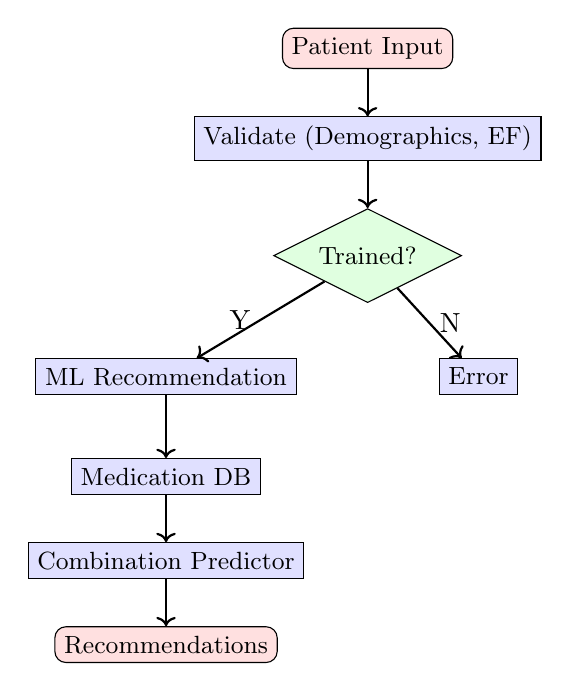
\begin{tikzpicture}[
  startstop/.style={rectangle, draw, fill=red!12, rounded corners, font=\small},
  process/.style={rectangle, draw, fill=blue!12, font=\small},
  decision/.style={diamond, draw, fill=green!12, aspect=2, font=\small},
  arrow/.style={->, thick},
  node distance=0.6cm
  ]
  \node[startstop] (s) {Patient Input};
  \node[process, below=of s] (v) {Validate (Demographics, EF)};
  \node[decision, below=of v] (t) {Trained?};
  \node[process, below left=1cm and 0.3cm of t] (ml) {ML Recommendation};
  \node[process, below right=1cm and 0.3cm of t] (err) {Error};
  \node[process, below=0.8cm of ml] (db) {Medication DB};
  \node[process, below=of db] (cb) {Combination Predictor};
  \node[startstop, below=of cb] (out) {Recommendations};
  \draw[arrow] (s) -- (v);
  \draw[arrow] (v) -- (t);
  \draw[arrow] (t) -- node[left] {Y} (ml);
  \draw[arrow] (t) -- node[right] {N} (err);
  \draw[arrow] (ml) -- (db);
  \draw[arrow] (db) -- (cb);
  \draw[arrow] (cb) -- (out);
\end{tikzpicture}
\caption{Recommendation pipeline with validation gate.}
\label{fig:flow}
\end{figure}

\subsection{Clinical Data Pipeline}
Figure~\ref{fig:dataflow} illustrates document-to-database flow: PDFs or images are processed by OCR (Tesseract/EasyOCR), then prescription and lab report parsers extract structured fields. The temporal PDF parser aggregates multi-page documents into time-series labs and vitals, stored in the clinical patient database (SQLite) with tables for patients, lab\_values, vital\_signs, medication\_history, clinical\_events, predictions, outcomes, calibrated\_parameters, and audit\_log. Each lab or vital entry is stored with a timestamp, value, unit, and an optional validation flag so that downstream models and the digital twin can use only validated points if desired. The upload API accepts multipart PDFs and returns a summary of extracted entities and any parsing errors, enabling the user to correct or re-upload if needed.

\begin{figure}[t]
\centering
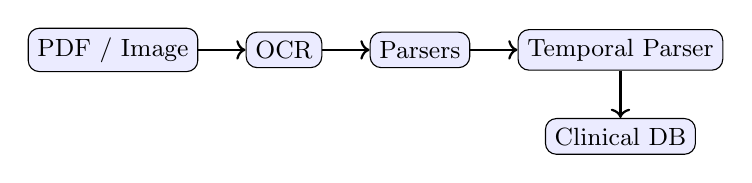
\begin{tikzpicture}[
  node distance=0.4cm and 0.6cm,
  box/.style={draw, rounded corners, fill=blue!8, font=\small},
  arrow/.style={->, thick}]
  \node[box] (p) {PDF / Image};
  \node[box, right=of p] (o) {OCR};
  \node[box, right=of o] (r) {Parsers};
  \node[box, right=of r] (t) {Temporal Parser};
  \node[box, below=0.6cm of t] (d) {Clinical DB};
  \draw[arrow] (p) -- (o);
  \draw[arrow] (o) -- (r);
  \draw[arrow] (r) -- (t);
  \draw[arrow] (t) -- (d);
\end{tikzpicture}
\caption{Clinical document and temporal data pipeline.}
\label{fig:dataflow}
\end{figure}

\subsection{Digital Twin and Mechanistic Calibration}
The digital twin component stores patient state, runs a patient-specific calibrator, and updates from outcomes. The Windkessel model is used with ODE: $dP/dt = (CO(t) - P/R)/C$, where $P$ is pressure, $CO$ is cardiac output, $R$ is systemic vascular resistance, and $C$ is arterial compliance. The calibrator fits $R$ and $C$ to patient history (e.g., pressure/CO or proxy variables) via scipy.optimize; after observed outcomes, parameters are updated to reduce prediction error, implementing a simple form of continuous learning.

\subsection{Digital Twin Lifecycle}
The digital twin lifecycle is: (1) \emph{Initialize}---register the patient with demographics and baseline data; optionally calibrate Windkessel parameters if enough history exists. (2) \emph{Recommend}---request recommendations; the engine uses the base ML recommender and applies patient-specific adjustments from the calibrated model where available. (3) \emph{Observe}---when an outcome is observed (e.g., follow-up EF, event), the client calls the update-outcome endpoint with the actual outcome and the prediction that was made. (4) \emph{Update}---the calibrator updates R and C (or other parameters) to reduce prediction error, and the updated parameters are stored for the next recommendation. This loop closes the gap between population-level ML and individual physiology and supports continuous improvement as more data accumulate.

\subsection{Validation and Input Requirements}
Before any recommendation or comparison is returned, the API checks: (i) the underlying ML model is loaded and marked as trained (\texttt{is\_trained}); (ii) required patient fields are present (at minimum age and ejection fraction for HF recommendations); (iii) for treatment comparison, at least one scenario with at least one medication is provided. If any check fails, the server responds with HTTP 400 and a JSON message describing the missing or invalid input. The frontend performs the same checks client-side to reduce invalid requests and to display inline validation errors. This two-layer validation ensures that the system never returns plausible-looking but unsupported recommendations when the model is cold or data are incomplete.

\subsection{Clinical Database Schema}
The clinical patient database (SQLite) stores longitudinal and audit data. Table~\ref{tab:schema} lists the core tables and their role. The \texttt{patients} table holds demographics, comorbidities, and data quality flags; \texttt{lab\_values} and \texttt{vital\_signs} store time-stamped series with units and validation flags. \texttt{medication\_history}, \texttt{clinical\_events}, \texttt{predictions}, and \texttt{outcomes} support the digital twin lifecycle. \texttt{calibrated\_parameters} stores Windkessel R and C (or other parameters) per patient and version. \texttt{audit\_log} records who performed which action and when; \texttt{documents} stores references to uploaded PDFs or images. This schema supports both one-off recommendations and ongoing digital twin updates as new data and outcomes arrive.

\begin{table}[t]
\caption{Clinical DB Core Tables}
\label{tab:schema}
\centering
\footnotesize
\begin{tabular}{@{}p{0.36\columnwidth}p{0.60\columnwidth}@{}}
\toprule
\textbf{Table} & \textbf{Purpose} \\
\midrule
patients & Demographics, comorbidities, quality flags \\
lab\_values & Time-series labs (value, unit, validated) \\
vital\_signs & Time-series vitals \\
medication\_history & Past and current medications \\
clinical\_events & Events and outcomes \\
predictions & Model ID, inputs, outputs, time \\
outcomes & Observed vs predicted \\
calibrated\_parameters & R, C per patient/version \\
audit\_log & Actor, action, timestamp \\
documents & Uploaded file references \\
\bottomrule
\end{tabular}
\end{table}

\section{Implementation}

\subsection{Backend Components}
Table~\ref{tab:backend} summarizes backend modules. The API is implemented in Python with FastAPI; models are persisted with joblib. The medication database queries the RxNorm API~\cite{rxnormapi} for concepts, properties, and interactions and caches results in SQLite. The recommendation router loads the personalized medication recommender (and optionally the enhanced recommender) at startup or on first use; the digital twin router instantiates the digital twin recommender with a path to the patient database. All routers share the same Pydantic models for \texttt{PatientInfo} and related DTOs to ensure consistency across endpoints. CORS is configured to allow the frontend origin so that the React app can call the API from the browser without cross-origin errors.

\begin{table}[t]
\caption{Backend Component Summary}
\label{tab:backend}
\centering
\footnotesize
\begin{tabular}{@{}p{0.28\columnwidth}p{0.68\columnwidth}@{}}
\toprule
\textbf{Component} & \textbf{Technology / Role} \\
\midrule
API & FastAPI, Pydantic, CORS \\
Med. Recommender & Random Forest (scikit-learn) \\
Effect Predictor & Gradient Boosting Regressor \\
Dosage Optimizer & scipy.optimize.minimize \\
Combo. Predictor & RF Regressor / guideline fallback \\
Patient Calibrator & Windkessel (R, C) + scipy \\
Clinical DB & SQLite: patients, labs, vitals, audit \\
Medication DB & RxNorm API + SQLite cache \\
OCR & Tesseract, EasyOCR \\
Parsers & Prescription, Lab, Temporal PDF \\
\bottomrule
\end{tabular}
\end{table}

\subsection{API Endpoints}
Table~\ref{tab:api} lists representative endpoints. Recommendations support both standard (category-level) and enhanced (drug-level with dosages and combination success) modes. Digital twin endpoints handle initialize, recommendations, update-outcome, status, and history. Temporal data endpoints support PDF upload and retrieval of labs/vitals/summary by patient. Medication endpoints provide search, category browse, detail lookup, combination prediction, and comparison.

\begin{table}[t]
\caption{API Endpoints by Domain}
\label{tab:api}
\centering
\footnotesize
\begin{tabular}{@{}p{0.26\columnwidth}p{0.70\columnwidth}@{}}
\toprule
\textbf{Domain} & \textbf{Endpoints} \\
\midrule
Recommendations & POST /recommendations, /enhanced, /compare \\
Digital Twin & POST /initialize, /recommendations, /update-outcome \\
Temporal Data & POST upload-pdf; GET labs, vitals, summary \\
Medications & GET search, category, name; POST predict, compare \\
\bottomrule
\end{tabular}
\end{table}

\subsection{Datasets and Features}
Training data are drawn from UCI Heart Failure~\cite{chicco2020uci}, Kaggle HF and BRFSS, and (when available) MIMIC-IV~\cite{johnson2016mimic}. Features include demographics (age, sex), vitals (heart rate, systolic and diastolic BP, SpO$_2$, temperature, respiratory rate), labs (ejection fraction, creatinine, sodium, hemoglobin, BNP, glucose, CPK, cholesterol), comorbidities (diabetes, hypertension, anaemia, smoking), and medication history. Missing values are handled with median imputation plus missingness indicators so that the model can use absence of a lab as a signal. Table~\ref{tab:data} summarizes scale and usage. Feature engineering produces 50+ derived and raw features per patient for the ML pipeline; the same feature set is used for recommendation, effect prediction, and combination success prediction where applicable.

\begin{table}[t]
\caption{Data Sources and Scale}
\label{tab:data}
\centering
\footnotesize
\begin{tabular}{@{}p{0.22\columnwidth}rrp{0.42\columnwidth}@{}}
\toprule
\textbf{Source} & \textbf{N} & \textbf{Feat.} & \textbf{Use} \\
\midrule
UCI HF & 299 & 13 & Survival, baseline \\
Kaggle HF & 918 & 12 & Clinical outcomes \\
Kaggle BRFSS & 253,680 & 21 & Demographics, comorbidities \\
MIMIC-IV & -- & Rich & Temporal (when available) \\
\bottomrule
\end{tabular}
\end{table}

\subsection{Frontend}
The frontend is a single-page React application (TypeScript) with a minimal navbar (Dashboard, Patients, Medications) and a dashboard that links to patient management, medication database, recommendations, digital twin, temporal data, predictions, and treatment comparison. Patient input is centralized in a reusable \texttt{PatientInfoForm}; recommendation results distinguish standard vs.\ enhanced (specific drugs, dosages, success rates). The UI is designed to avoid duplicate forms and to present a hospital-grade, professional layout.

\subsection{Model Formulation and Training}
The medication recommender trains one binary classifier per medication (or per category) using Random Forest; the positive class indicates that the medication was associated with benefit (e.g., prescribed and patient improved). The treatment effect predictor is a Gradient Boosting regressor that predicts change in ejection fraction, mortality risk, or readmission risk given patient features and medication. The dosage optimizer uses \texttt{scipy.optimize.minimize} to find doses that maximize predicted benefit subject to safety bounds. The combination success predictor is a Random Forest regressor trained on (patient features, medication set) $\mapsto$ success rate (0--1); when training data are insufficient, a guideline-based fallback assigns scores from evidence-based combination rules. Table~\ref{tab:hyper} summarizes representative hyperparameters used in training.

\begin{table}[t]
\caption{Representative Training Hyperparameters}
\label{tab:hyper}
\centering
\footnotesize
\begin{tabular}{@{}p{0.38\columnwidth}p{0.58\columnwidth}@{}}
\toprule
\textbf{Component} & \textbf{Setting} \\
\midrule
Random Forest (med., combo.) & n\_estimators=100, max\_depth=10 \\
Gradient Boosting (effect) & n\_estimators=100, learning\_rate=0.1 \\
Train/validation split & 80/20 stratified \\
Calibration (Windkessel) & L-BFGS-B, bounds on R, C \\
\bottomrule
\end{tabular}
\end{table}

\subsection{Medication Database and RxNorm Integration}
The medication database resolves drug names to RxNorm concept identifiers (RxCUI), retrieves properties (strength, form, mechanism, indications, contraindications), and caches results in SQLite. Heart-failure-relevant medication lists can be preloaded via \texttt{load\_heart\_failure\_medications}, which queries the RxNorm API for common HF drug names and stores them with dosage forms and strengths. Drug-drug interaction checks use the same cache and API. The frontend medication search calls \texttt{/medications/search} with autocomplete; the comparison page uses search to add medications to scenarios before calling \texttt{/compare}.

\subsection{Data and Feature Engineering}
Raw inputs (age, sex, vitals, labs, comorbidities, medications) are transformed into a fixed-length feature vector for the ML models. Demographics are one-hot or scaled as appropriate; vitals and labs are normalized and missing values are replaced with the training-set median plus a binary missing indicator. Comorbidities are binary flags. Medication history is encoded as binary indicators per drug or category. The same pipeline is applied at inference time so that training and serving use identical feature semantics. For the combination success predictor, the feature vector is augmented with the set of medication identifiers (or their embeddings) for the proposed combination; the model then predicts a scalar success rate and optional outcome deltas (e.g., EF change). This allows the system to compare multiple combinations for the same patient and rank them by predicted success.

\subsection{API Design and Contract}
All endpoints use JSON for request and response bodies. Request schemas are defined with Pydantic so that invalid types or missing required fields are rejected before reaching business logic. Response schemas include a consistent structure for errors: \texttt\{\texttt{"detail"}: \textit{message}\} for HTTP 4xx/5xx. Successful recommendation responses include \texttt{recommendations} (list of suggested medications with scores or details), \texttt{specific\_recommendations} (for enhanced: drug name, strength, form, dosage, frequency, combination success rate), and optional \texttt{expected\_outcomes}. The compare endpoint returns a list of scenarios with \texttt{success\_rate}, \texttt{medication\_names}, and \texttt{total\_benefit} for each. This contract allows the frontend to render standard and enhanced results without branching on endpoint type. The shared \texttt{PatientInfo} schema includes required fields (e.g., \texttt{age}, \texttt{ejection\_fraction}) and optional vitals, labs, and comorbidities; the API documents which endpoints require which subset so that clients can validate before sending.

\section{Evaluation and Results}

\subsection{Validation and Safety}
The system enforces server- and client-side validation: recommendations and comparison endpoints require a trained model and complete required patient fields (e.g., age, ejection fraction). If not satisfied, the API returns HTTP 400 with a clear message rather than synthetic recommendations. This design eliminates the risk of presenting mock or placeholder results as clinical advice. Table~\ref{tab:validation} lists the main validation checks applied at the API layer.

\begin{table}[t]
\caption{API-Layer Validation Checks}
\label{tab:validation}
\centering
\footnotesize
\begin{tabular}{@{}p{0.30\columnwidth}p{0.66\columnwidth}@{}}
\toprule
\textbf{Endpoint / Flow} & \textbf{Conditions Enforced} \\
\midrule
Recommendations & \texttt{is\_trained}; age, EF present; non-empty recs. \\
Compare scenarios & \texttt{is\_trained}; age present; $\ge$1 scenario, $\ge$1 med each \\
Digital twin init & Valid patient\_id, patient\_info \\
Enhanced recommendations & Same as recommendations + medication DB available \\
\bottomrule
\end{tabular}
\end{table}

\subsection{System Complexity}
Table~\ref{tab:complexity} summarizes the technical complexity. The platform spans multiple ML models (classification and regression), mechanistic ODE models with calibration, two SQLite databases (clinical and medication), external API integration (RxNorm), document processing (OCR and parsing), and a full REST API and web UI. The digital twin loop (initialize $\rightarrow$ recommend $\rightarrow$ observe outcome $\rightarrow$ update) is implemented end-to-end.

\subsection{Component and Endpoint Coverage}
Each major backend capability is exposed via REST and is reachable from the frontend: recommendations (standard and enhanced), treatment comparison, digital twin (initialize, status, history, recommendations, update-outcome), temporal data (upload, labs, vitals, summary), medication search and combination prediction, and predictions/trajectories. The dashboard and Patients page provide a single entry point to these features without duplicating patient entry forms; the Medications page provides search, category browse, and detail views backed by the same medication API. Table~\ref{tab:frontend} maps main frontend pages to the primary backend domains they use; all rely on the shared API client and, where applicable, the shared \texttt{PatientInfoForm} for consistent input capture.

\begin{table}[t]
\caption{Frontend Pages and Backend Domains}
\label{tab:frontend}
\centering
\footnotesize
\begin{tabular}{@{}p{0.32\columnwidth}p{0.64\columnwidth}@{}}
\toprule
\textbf{Page} & \textbf{Primary API Domain(s)} \\
\midrule
Dashboard & (navigation only) \\
Patients & Digital twin, temporal, recommendations \\
Recommendations & Recommendations (std/enhanced) \\
Treatment Comparison & Compare combinations \\
Digital Twin & Digital twin (all) \\
Temporal Data & Temporal data (upload, labs, vitals) \\
Predictions & Predictions, trajectories \\
Medication Database & Medications (search, category, load) \\
\bottomrule
\end{tabular}
\end{table}

\begin{table}[t]
\caption{Technical Complexity Overview}
\label{tab:complexity}
\centering
\footnotesize
\begin{tabular}{@{}p{0.22\columnwidth}p{0.74\columnwidth}@{}}
\toprule
\textbf{Layer} & \textbf{Elements} \\
\midrule
ML & Med. recommender, effect predictor, dosage optimizer, combo. predictor \\
Mechanistic & Windkessel; R/C calibration; outcome-based update \\
Data & Clinical DB (10+ tables), medication DB, registry \\
Document & OCR (Tesseract, EasyOCR); prescription/lab/temporal parsers \\
API & 7 routers, 30+ endpoints, Pydantic schemas \\
Frontend & 8+ pages, shared forms, dashboard navigation \\
\bottomrule
\end{tabular}
\end{table}

\subsection{Alignment with Clinical Workflows}
The workflow supports: (1) registering a patient and initializing the digital twin; (2) uploading documents to populate temporal labs/vitals; (3) requesting recommendations (standard or enhanced) and treatment comparisons; (4) recording outcomes and updating the twin. Audit logging and structured error responses support accountability and debugging. No feature returns synthetic or placeholder data when preconditions are not met, aligning with the requirement that the system be trustworthy in pilot or research deployments.

\subsection{Example End-to-End Scenario}
A clinician opens the Dashboard, navigates to Patients, and creates a new patient with age, ejection fraction, and key labs. She then goes to Digital Twin and initializes the twin for this patient; the system stores the record and, if enough history exists, calibrates Windkessel parameters. Next, she requests enhanced recommendations: the API validates that the model is trained and that age and EF are present, then returns specific drugs (e.g., sacubitril/valsartan 24/26\,mg twice daily), dosages, and a combination success rate. She can also open Treatment Comparison, add two scenarios (e.g., scenario A: ACE-i + beta-blocker; scenario B: ARNI + beta-blocker) using the medication search, and receive success rates and expected outcomes for each. Later, after a follow-up visit, she records the observed outcome via the update-outcome endpoint so that the digital twin can adapt for the next recommendation cycle.

\section{Discussion}

\subsection{Limitations}
Models are trained on public datasets (UCI, Kaggle); performance in real clinical settings would require validation on local EHR data. The combination success predictor can fall back to guideline-based heuristics when training data are scarce. OCR and parsing accuracy depend on document quality and layout. The current Windkessel calibration uses limited signals; richer hemodynamic data would improve personalization. The medication database relies on RxNorm only; integration with DrugBank or other sources would require additional licensing and schema mapping.

\subsection{Interpretability and Explainability}
The Windkessel component provides a physically interpretable layer: clinicians can inspect calibrated R and C and relate them to vascular resistance and compliance. The ML recommenders are tree-based (Random Forest, Gradient Boosting), which allow feature-importance and partial dependence analysis for post hoc explanation. The API does not yet expose explanation endpoints; adding SHAP or similar would support transparency in a clinical setting.

\subsection{Regulatory and Deployment Considerations}
For use in regulated environments, the platform would need: (i) formal validation and possibly regulatory clearance depending on jurisdiction; (ii) access control and authentication integrated with hospital identity providers; (iii) audit logs retained and exportable for inspections. The current implementation provides audit logging and structured errors as a foundation; authentication and role-based access would be added in a production deployment.

\subsection{Performance and Scalability}
The API is designed for low to moderate throughput: recommendation and comparison calls are CPU-bound (model inference and database lookups). For higher load, the API can be run behind a reverse proxy (e.g., nginx) with multiple workers; the SQLite databases can be replaced with PostgreSQL or another RDBMS and connection pooling. The RxNorm API is called on cache miss; aggressive caching of medication lookups keeps external calls low. Frontend assets are static and can be served via a CDN. No formal load testing results are reported here; they are left for future work when deployment targets are fixed.

\subsection{Comparison with Related Systems}
Table~\ref{tab:comparison} situates our platform against typical characteristics of CDSS and digital twin systems. Unlike pure guideline checklists, we provide data-driven and mechanistic predictions with drug-level and combination-level output. Unlike black-box ML-only systems, we expose a calibrated physiological layer (Windkessel) and enforce strict validation so that no synthetic recommendations are ever returned. Unlike document systems that only archive PDFs, we parse and store temporal labs and vitals for use in the digital twin and recommendations. The combination of these aspects in a single deployable stack is a distinguishing feature of the HF-Digital Twin Platform.

\begin{table}[t]
\caption{Comparison with Related System Types}
\label{tab:comparison}
\centering
\footnotesize
\begin{tabular}{@{}p{0.28\columnwidth}p{0.68\columnwidth}@{}}
\toprule
\textbf{Aspect} & \textbf{HF-Digital Twin vs.\ Others} \\
\midrule
Recommendations & Drug-level + dosages; combo. success; not mock when untrained \\
Digital twin & Calibrated Windkessel; outcome-based updates \\
Data ingestion & OCR + parsers $\to$ temporal DB (not only archive) \\
Validation & Server + client; HTTP 400 on missing/invalid \\
Deployment & REST API + React UI; single-column tables in paper \\
\bottomrule
\end{tabular}
\end{table}

\subsection{Reproducibility and Threats to Validity}
The codebase is structured so that data loading, feature engineering, training, and API can be run from scripts and configuration. Datasets (UCI, Kaggle) are publicly available; MIMIC-IV requires institutional access. Model checkpoints (e.g., \texttt{.pkl}) are saved after training so that the same model can be loaded in the API. A threat to validity is that reported complexity and workflow alignment are based on the implemented system rather than a user study; future work should include formative evaluation with clinicians. Another threat is that combination success and effect predictions have not been validated on held-out clinical trials or EHR cohorts in this paper; such validation is planned as part of future work.

\subsection{Future Work}
Planned extensions include: integration with more drug knowledge bases (e.g., DrugBank when licensing permits), survival and trajectory models, external validation on MIMIC-IV and partner sites, optional deployment with containerized services (Docker) for scalability, explanation APIs (e.g., SHAP) for recommended medications and combination scores, and formative usability studies with clinicians to refine workflows and presentation.

\section{Conclusion}

We presented the HF-Digital Twin Platform, a hybrid mechanistic--ML system for personalized heart failure medication recommendations. The platform combines data-driven models (Random Forest, Gradient Boosting) with a calibrated Windkessel-based digital twin, an RxNorm-backed medication database, combination success prediction, and a clinical document pipeline from PDFs to temporal patient data. Strict validation ensures that untrained models or incomplete inputs never produce fictitious recommendations. The architecture, API, and frontend are implemented and documented to support reproducibility and further research toward guideline-aligned, personalized HF care.

The paper detailed the end-to-end design: high-level architecture, recommendation and data pipelines, clinical database schema, model formulation and training, API and validation strategy, and evaluation of complexity and workflow alignment. All tables were formatted to fit within a single column to avoid cross-column overflow in the two-column IEEE layout. Figures (architecture, recommendation flowchart, data pipeline) were drawn with TikZ and kept compact for the same reason.

We hope this technical description enables other groups to replicate or extend the system and to adapt it for local datasets and regulatory contexts. Future work will focus on external validation on held-out EHR or trial data, usability studies with clinicians, and optional deployment patterns (e.g., Docker, cloud) for pilot sites.

\section*{Acknowledgment}
The authors thank the open-source communities behind FastAPI, scikit-learn, RxNorm, and the UCI/Kaggle/MIMIC data providers. This work was conducted as part of a research and development effort on digital twins for heart failure; no external funding is acknowledged here.

\paragraph{Data and Code Availability.}
The system is implemented in a single repository containing the \texttt{pdt} Python package (backend), React frontend, and documentation. Public datasets (UCI Heart Failure, Kaggle) are cited in the references; MIMIC-IV access is subject to institutional agreement. Trained model artifacts can be reproduced using the provided training scripts and the same datasets.

\bibliographystyle{IEEEtran}
\bibliography{references}

\end{document}
